\documentclass{beamer}
\usepackage[latin1]{inputenc}
\usepackage{tikz}
\usepackage{makecell}
\usepackage{pgfplots}
\usepackage{pgfplotstable} 
\usepackage{bchart}
%\pgfplotsset{compat=1.12}
\usepackage{sansmath}
\usetheme{texsx}
\usetikzlibrary{
	arrows.meta,
	chains,
	decorations.pathreplacing,
	automata,
	positioning,
	scopes,
	quotes,
	shapes,
	shadows	
}
\title{Fast Decompression Lucene Codec}
\author{Ivan Mamontov imamontov@griddynamics.com}
\institute{Berlin Buzzwords}
\date{Jun 1st, 2015}

\addtobeamertemplate{navigation symbols}{}{%
    \usebeamerfont{footline}%
    \usebeamercolor[black]{footline}%
    \hspace{6em}%
    \insertframenumber/\inserttotalframenumber
}


\pgfplotstableread[col sep=comma]{
a,b,c,d,e
128,  82.638  ,200.452 ,194.441  ,330.123  
256,  139.914 ,261.881 ,346.855  ,583.440  
512,  225.505 ,341.506 ,592.312  ,1046.636 
1024, 396.605 ,518.709 ,1100.371 ,2149.478 
2048, 743.370 ,868.560 ,2089.506 ,4058.115 
4096, 1436.633,1557.861,4204.929 ,8023.846 
8192, 2827.855,2953.913,7758.365 ,14458.539
16384,5654.820,5779.984,14938.887,25235.819
}\mytable

\AtBeginSection{\frame{\sectionpage}}
\setbeamertemplate{section page}[mine]
\setbeamertemplate{subsection page}[mine]

\newcommand\hugefont{\fontsize{36}{42.2}\selectfont}

\begin{document}
	%\begin{frame}
	%	\titlepage
	%\end{frame}
{
\usebackgroundtemplate{}
    \begin{frame}[plain]
        \begin{tikzpicture}[remember picture,overlay]
            \node[at=(current page.center)] {
                \includegraphics[keepaspectratio=true,height=\paperheight]{resources/Logo.png}
            };
        \end{tikzpicture}
     \end{frame}
}
	\begin{frame}
    		\begin{itemize}
    			\frametitle{About me}
    		    \item Software engineer at Grid Dynamics
    		    \item I am interested in low-level system programming
		\end{itemize}
  	\end{frame}
  	\begin{frame}
  		\frametitle{Table of Contents}
  		\tableofcontents
  	\end{frame}
  	\section{Compression in Lucene}
  	\begin{frame}
		\frametitle{Requirements of a search index}
		\begin{itemize}
		\item compress index as possible
			\begin{itemize}
			\item minimize I/O
			\item minimize index size
			\item FS/Memory/CPU cache friendly
			\end{itemize}
		\item avoid disc seeks
			\begin{itemize}
				\item disc seek is $\approx10$ms 
			\end{itemize}						
		\end{itemize}
  	\end{frame}	
  	\begin{frame}
  		\frametitle{The numbers every engineer should know}
  		\begin{itemize}
  		\item L1 cache reference 0.5 ns
  		\item Branch mispredict 5 ns
  		\item L2 cache reference 7 ns
  		\item Main memory reference 100 ns
  		\item Read 1 MB sequentially from memory 250,000 ns
  		\item Disk seek 10,000,000 ns
  		\item Read 1 MB sequentially from disk 30,000,000 ns
  		\end{itemize}
  	\end{frame}
	\begin{frame}
		\frametitle{Codec API}
		\begin{center}
		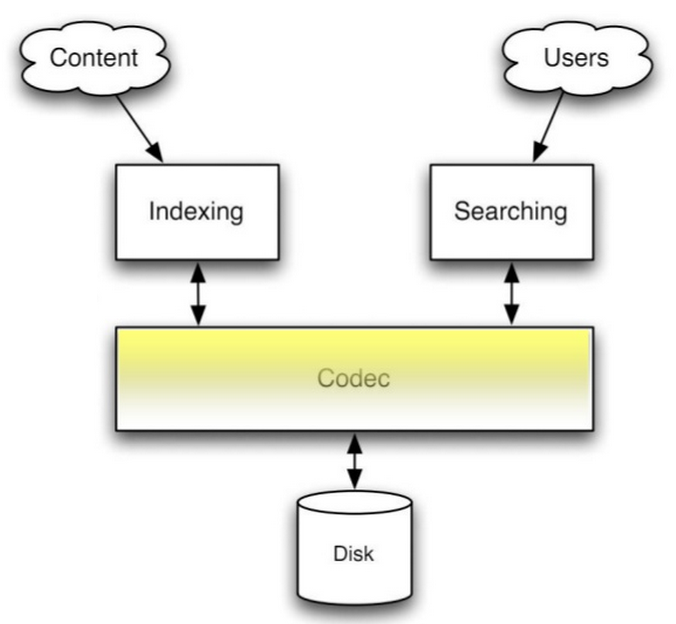
\includegraphics[keepaspectratio=true,height=.70\paperheight]{resources/codecAPI.png}
		\end{center}
 	\end{frame}	
 	\begin{frame}
 		\frametitle{4D Codec API}
 		\begin{center}
		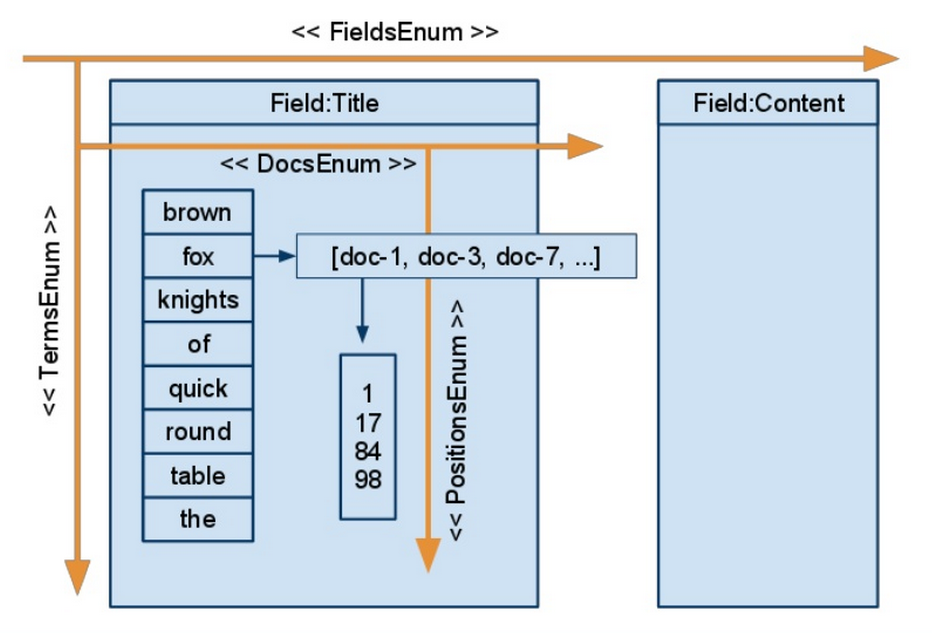
\includegraphics[keepaspectratio=true,height=.70\paperheight]{resources/4D.png}
		\end{center}
 	\end{frame}
  	\begin{frame}
  		\frametitle{Postings lists}
  		\begin{itemize}
  			\item Encoded using modified FOR delta
  			\begin{enumerate}
  			\item uses delta
  			\item splits into block of N=128 values
  			\item bit packing per block
  			\item remaining docs, encode with vint
  			\end{enumerate}
  			\vskip15pt 
  			Example with N=4\hspace{1cm}1,3,4,6,8,20,22,26,30,158\\
  			\hspace*{4.1cm}1,2,1,2,2,12,2,4,4,128\\
			\hspace*{4.1cm}[1,2,1,2] [2,12,2,4] 4,128\\
  		\end{itemize}
  	\end{frame}
  	\begin{frame}
  		\frametitle{What is FOR encoding?}
  		To encode the following 4 numbers 1, 2, 1, 2:
		\vskip15pt 
  		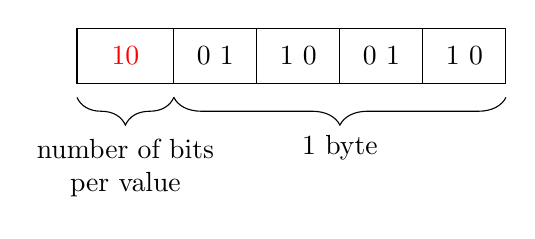
\begin{tikzpicture}[
 		      	start chain = going right,
     			node distance = 0pt,
				ArrayStyle/.style={draw, minimum width=3.5em, minimum 									height=2em, outer sep=0pt, on chain}]		
			\node [ArrayStyle] (1) {{\color{red!100}10}};
			\node [ArrayStyle, minimum width=3em] (2) {0 1};
			\node [ArrayStyle, minimum width=3em] (3) {1 0};
			\node [ArrayStyle, minimum width=3em] (4) {0 1};
			\node [ArrayStyle, minimum width=3em] (5) {1 0};	
			\draw[decorate,decoration={brace, amplitude=10pt, 					raise=5pt, mirror}]
  				(2.south west) to node[black,midway,below= 15pt] 				{1 byte} (5.south east);
			\draw[decorate,decoration={brace, amplitude=10pt, 					raise=5pt, mirror}]
  				(1.south west) to node[black,midway,below= 15pt] 				{\makecell[c]{number of bits\\per value}} (1.south east);
		\end{tikzpicture} 
		\vskip15pt 	
		FOR requires 1 byte instead of $4*4=16$ bytes!
  	\end{frame}
  	\begin{frame}
  		\frametitle{What is FOR encoding?}
  		\begin{itemize}
    		    \item pros
    		    \begin{itemize}
    		    		\item great compression rate % Up to 2 times faster than in variable-byte encoding
    		    		\item fast decoding speed
    		    		\item \textbf{can be vectorized}
    		    \end{itemize}
    		    \item cons
    		    \begin{itemize}
    		    		\item no random access within the block
    		    		\item the cost is determined by the largest delta in a block
    		    \end{itemize}
		\end{itemize}  		
  	\end{frame}
  	\section{Scalar vs. Vectors}
  	\begin{frame}[fragile=singleslide]
  		%Let us explain this with an example:
  		%The code in example 1b can be reduced to just 4 machine instructions if the
		%instruction set AVX or higher is enabled. The SSE2 instruction set will give 8
		%machine instructions because the maximum vector register size is half as big for
		%instruction sets prior to AVX. The code in example 1a will generate approximately
		%44 instructions if the compiler does not automatically vectorize the code.
    		\frametitle{Scalar vs. Vectors}
		\begin{verbatim}
float a[4], b[4], c[4];       
...
for (int i = 0; i < 4; i++) { 
 c[i] = a[i] + b[i];     
}
		\end{verbatim}
		\begin{itemize}
			\item JIT $\approx32$ machine instructions
			\item gcc $\approx24$ machine scalar instructions
			\item gcc -- 4 machine instructions with SSE2			
		\end{itemize}
  	\end{frame}  
  	\begin{frame}
%With conventional scalar operations, four add instructions must be executed one after another to obtain the sums as shown
    		\frametitle{Scalar vs. Vectors}
  		\tikzset{% define the style of the nodes for drawing the squares
     		mysquare/.style={shape=rectangle,draw=black!                       			100,thick,top color=white}
   		}
		\begin{columns}[T] % align columns
		\begin{column}{.48\textwidth}
  		\begin{tikzpicture}
    			\foreach \x in {0,...,3} {% loop over the three rows
       		\node[mysquare] at (0,-\x) {$A_\x$};
       		\node at (1,-\x) {$+$};
       		\node[mysquare] at (2,-\x) {$B_\x$};
       		\node at (3,-\x) {$=$};
       		\node[mysquare] at (4,-\x) {$C_\x$};
    			}
		 \end{tikzpicture}
		 \end{column}
		 \begin{column}{.48\textwidth}
		    \begin{tikzpicture}% use positioning to put the boxes together
    				\foreach \letter/\col/\x in {A/yellow!30/0, B/green!40/2, C/red!50/4} {
      				\node[mysquare=\col] (\letter 0) at (\x,0){$\letter_0$};
      				\node[below=-1pt of \letter 0,mysquare=\col] (\letter 1) {$\letter_1$};
      				\node[below=-1pt of \letter 1,mysquare=\col] (\letter 2) {$\letter_2$};
      				\node[below=-1pt of \letter 2,mysquare=\col] (\letter 3) {$\letter_3$};
    				}
    				\node at (1,-0.8) {$+$};% place + and = by hand
    				\node at (3,-0.8) {$=$};
  			\end{tikzpicture}
		 \end{column}
		 \end{columns}
  	\end{frame}

  	\begin{frame}
    		\frametitle{Scalar vs. Vectors}
    		\begin{itemize}
    			\item 75\% fewer loads
    		    	\item 75\% fewer adds
    		    	\item 75\% fewer stores
		\end{itemize}
  	\end{frame}  	
  	\begin{frame}
  		
  	\end{frame}
  	\begin{frame}
  		\frametitle{Vectorization in HotSpot}
  		%Sometimes it is possible to move the kernel to C/C++, use SIMD there and call via JNI. However, the cost of the JNI call can be significant as are the difficulties of ensuring memory is properly aligned for SIMD execution
  		%In HotSpot versions beginning with Java 7u40, the server compiler provides support for auto-vectorisation. According to JDK-6340864
		%However, this seems to be true only for "simple loops" - at least for the moment. For example, accumulating an array cannot be vectorised yet JDK-7192383
		\begin{itemize}
		\item auto-vectorization -- vector arithmetic is not supported yet. Only array initialization and array copy.
  		\begin{itemize}
  			\item \url{http://bugs.java.com/view_bug.do?bug_id=6340864}
  			\item \url{http://bugs.java.com/view_bug.do?bug_id=7192383}
  		\end{itemize}
  		\item explicit vectorization -- JVM does not provide interfaces
		\end{itemize}
  	\end{frame}
  	\begin{frame}
  	  	\frametitle{Workaround}
  	  	\begin{itemize}
  	  	\item write kernel code in C/C++
  	  	\item call via JNI
  	  	\end{itemize}
  	  	\pause
  	  	\vskip15pt 
  	  	The cost of the JNI call can be significant.
  	\end{frame}
  	\begin{frame}
  		\frametitle{What makes JNI calls slow?}
  		\begin{itemize}
  			\item {\color{gray} Wrap object references to JNI handles.}
  			\item {\color{gray} Obtain JNIEnv*, jclass/jobject and pass them as parameters.}
  			\item {\color{gray} Lock an object monitor if the method is synchronized.}
  			\item \textbf{Call the native function.}
  			\item {\color{gray} Check if safepoint is needed.}
  			\item {\color{gray} Unlock monitor if locked.}
  			\item {\color{gray} Unwrap object result and reset JNI handles block.}
  			\item {\color{gray} Handle JNI exceptions.}
  		\end{itemize}
  	\end{frame}
  	\section{Java Critical Native}	
  	\begin{frame}
  		\frametitle{JDK-7013347 Critical Native}
  		Critical native looks like JNI method:
  		\begin{itemize}
  			\item static and not synchronized
  			\item not throw exceptions
  			\item does not use wrappers
  			\item works with primitives
  		\end{itemize}
  		\vskip15pt
  		See details in JDK-7013347
  	\end{frame}
	\section{Benchmarks}
	\begin{frame}
		\frametitle{Native FOR}
		A simple C library for compressing lists of integers \url{https://github.com/lemire/simdcomp} (thanks to  Daniel Lemire, Leonid Boytsov)
		\begin{itemize}
		\item supports SSE2, SSE4.1, AVX 
		\item uses C99 syntax
		\item uses SIMD intrinsics
		\end{itemize}
	\end{frame}
	\begin{frame}
		\frametitle{Microbenchmark}
		\begin{itemize}
		\item java code
		\begin{itemize}
		\item java\_vint -- classic vint implementation
		\item java\_FOR -- classic FOR implementation
		\end{itemize}
		\item JNI + native FOR implementation
		\begin{itemize}
		\item normal\_JNI -- usual JNI call
		\item critical\_JNI -- critical native call
		\end{itemize}
		\end{itemize}
		Environment
			\begin{itemize}
				\item i5-4300M CPU @ 2.60GHz (Haswell)
				\item fedora 21 (kernel 3.17.4)
				\item JRE 1.8.0\_40
				\item gcc 4.9.2 
			\end{itemize}
		\vskip15pt
		Decodes blocks with fixed size\\
		Every block contains random elements with fixed density
	\end{frame}
  	\begin{frame}
  		\frametitle{Microbenchmark}
  			%The vectorized version is roughly twice as fast as the scalar version
			\begin{tikzpicture}
			\pgfkeys{/pgf/number format/.cd,use comma,1000 sep={},}
    			\begin{loglogaxis}[
            		log basis x=2,log basis y=2,
            		%label style={font=\tiny},
            		xlabel={Block size},ylabel={Decoding latency, ns/op},
            		legend entries={critical\_JNI, normal\_JNI, java\_FOR, java\_vbyte},
            		xmin=96,xmax=24576,
            		ymin=60,ymax=30720,
            		separate axis lines,
            		axis x line*=bottom,
            		axis y line*=left,
            		axis line style={draw=gray!50},
            	ytick={60,120,240,480,960,1920,3840,7680,15360,30720},           			xtick={96,192,384,768,1536,3072,6144,12288, 24576},
            		yticklabel={\pgfkeys{/pgf/fpu}\pgfmathparse{60*(2^(\ticknum))}%
                        \pgfmathprintnumber[fixed,precision=0]\pgfmathresult%
                        \pgfkeys{/pgf/fpu=false}%
                        },
		            xticklabel={\pgfkeys{/pgf/fpu}\pgfmathparse{2^(7+\ticknum)}%
                        \pgfmathprintnumber[fixed]\pgfmathresult%
                        \pgfkeys{/pgf/fpu=false}%
                        },
            x tick label as interval,
            ymajorgrids,
            tick align=outside,
            legend style={draw=none,fill=none,
                          at={(axis description cs:1.0,0.5)}, 
                          anchor=west,
                          %nodes={font=\tiny}
                          },
            tick label style={font=\tiny}
        ]
        			\addplot[red,very thick,mark=square*]     table[x=a,y=b] {\mytable};    
        			\addplot[green,very thick,mark=triangle*] table[x=a,y=c] {\mytable};    
        			\addplot[blue,very thick,mark=diamond*]   table[x=a,y=d] {\mytable}; 
        			\addplot[orange,very thick,mark=*]        table[x=a,y=e] {\mytable}; 
    			\end{loglogaxis}
		\end{tikzpicture}
	\end{frame}  	
	\begin{frame}
		\frametitle{SIMD codec}
		\begin{itemize}
		    \item based on Lucene50 codec
		    \item uses \url{https://github.com/lemire/simdcomp} as native FOR implementation
			\item still in progress so it does not support
			\begin{itemize}
				\item freqs
				\item positions
				\item offsets
				\item payloads
			\end{itemize}			
		\end{itemize}
		Source code available at \url{http://git.io/vkY1o}
	\end{frame}
	\begin{frame}
		\frametitle{Lucene benchmark}
		\begin{itemize}
			\item indexes all of Wikipedia's English XML export
				\begin{itemize}
					\item only documents are indexed: term frequencies and positions are omitted
					\item one large segment is used(about 1GB)
				\end{itemize}
			\item measures how long it takes to search top 10K frequent terms
			\item environment
			\begin{itemize}
				\item i5-4300M CPU @ 2.60GHz (Haswell)
				\item fedora 21 (kernel 3.17.4)
				\item JRE 1.8.0\_40
				\item gcc 4.9.2 
			\end{itemize}
			\item ant run-task -Dtask.alg=conf/searchOnlyWiki.alg -Dtask.mem=8G
		\end{itemize}
	\end{frame}
	\begin{frame}
		\frametitle{Benchmark results}
		\begin{center}
  		\begin{bchart}[step=5,min=30,max=65,unit=s]
        		\bcbar[label=SIMDCodec]{49}
            \smallskip
        		\bcbar[label=Lucene50]{60}
            \smallskip
    		\end{bchart}
		\end{center}
	\end{frame}
	\begin{frame}
		\frametitle{Future work}
		\begin{itemize}
			\item Fast compression and intersection of lists of sorted integers \url{https://github.com/lemire/SIMDCompressionAndIntersection}
			\item Fast decoder for VByte-compressed integers \url{https://github.com/lemire/MaskedVByte}
			\item Native roaring codec
			\item Native facet component
			\item Native docvalues decoder
		\end{itemize}
	\end{frame}
	\begin{frame}
		\hugefont
		\begin{center}
		Thank you!
		\end{center}
	\end{frame}
\end{document}